\documentclass[11pt]{article}

% Packages
\usepackage[utf8]{inputenc}
\usepackage[margin=1in]{geometry}
\usepackage{setspace}
\usepackage{graphicx}
\usepackage{hyperref}
\usepackage{amsmath}
\usepackage{cite}
\usepackage{float}
\usepackage{listings}
\usepackage{xcolor}

% Set line spacing to 1.5
\setstretch{1.5}

% Code listing settings
\lstset{
    basicstyle=\ttfamily\footnotesize,
    breaklines=true,
    frame=single,
    backgroundcolor=\color{gray!10},
    keywordstyle=\color{blue},
    commentstyle=\color{green!50!black},
    stringstyle=\color{red}
}

% Title information
\title{\textbf{Social Synchrony Analysis Using YOLO Pose Estimation}}
\author{
    Gilad Sarusi \\
    \textit{GitHub: @giladsar} \\
    \\
    Course Number: 001-2902-31 \\
    Date: February 22, 2026
}
\date{}

\begin{document}

% Cover Page
\maketitle
\thispagestyle{empty}
\newpage

% Set page numbering
\setcounter{page}{1}

% Introduction
\section{Introduction}

\subsection{Background}
Social synchrony refers to the temporal coordination of behaviors between individuals during social interactions. Understanding these patterns is crucial in fields such as psychology, neuroscience, and social sciences, as it provides insights into the quality and dynamics of interpersonal relationships. Traditionally, the analysis of social synchrony has relied on manual coding or sensor-based measurements, which can be time-consuming and limited in scope.

Recent advances in computer vision and deep learning have opened new possibilities for automated analysis of social interactions through video data. Pose estimation models, particularly the YOLO (You Only Look Once) family of models, have demonstrated remarkable accuracy in detecting and tracking human body movements in real-time.

\subsection{Research Motivation}
This project aims to leverage state-of-the-art pose estimation technology to quantify and analyze social synchrony in dyadic interactions. By extracting body movement patterns from video data and computing synchrony metrics, we can provide objective, quantitative measures of interpersonal coordination. This approach offers several advantages over traditional methods:

\begin{itemize}
    \item \textbf{Non-invasive}: Uses standard video recordings without requiring specialized sensors
    \item \textbf{Scalable}: Can process multiple videos efficiently
    \item \textbf{Comprehensive}: Captures full-body movement patterns
    \item \textbf{Reproducible}: Provides consistent, automated analysis
\end{itemize}

\subsection{Main Objectives}
The primary objectives of this project are:

\begin{enumerate}
    \item Implement a robust pose estimation pipeline using YOLO models for video analysis
    \item Develop algorithms for tracking multiple individuals across video frames
    \item Extract and preprocess body movement signals from pose keypoints
    \item Compute social synchrony metrics, including cross-correlation and co-crossing events
    \item Visualize and interpret synchrony patterns in dyadic interactions
\end{enumerate}

% Dataset Description
\section{Dataset Description}

\subsection{Examples of Data}
The dataset consists of video recordings of dyadic interactions. Sample frames from the analyzed video are shown in Figure~\ref{fig:sample_frames}. These frames demonstrate the pose estimation output, with detected keypoints overlaid on the original video frames.

\begin{figure}[H]
    \centering
    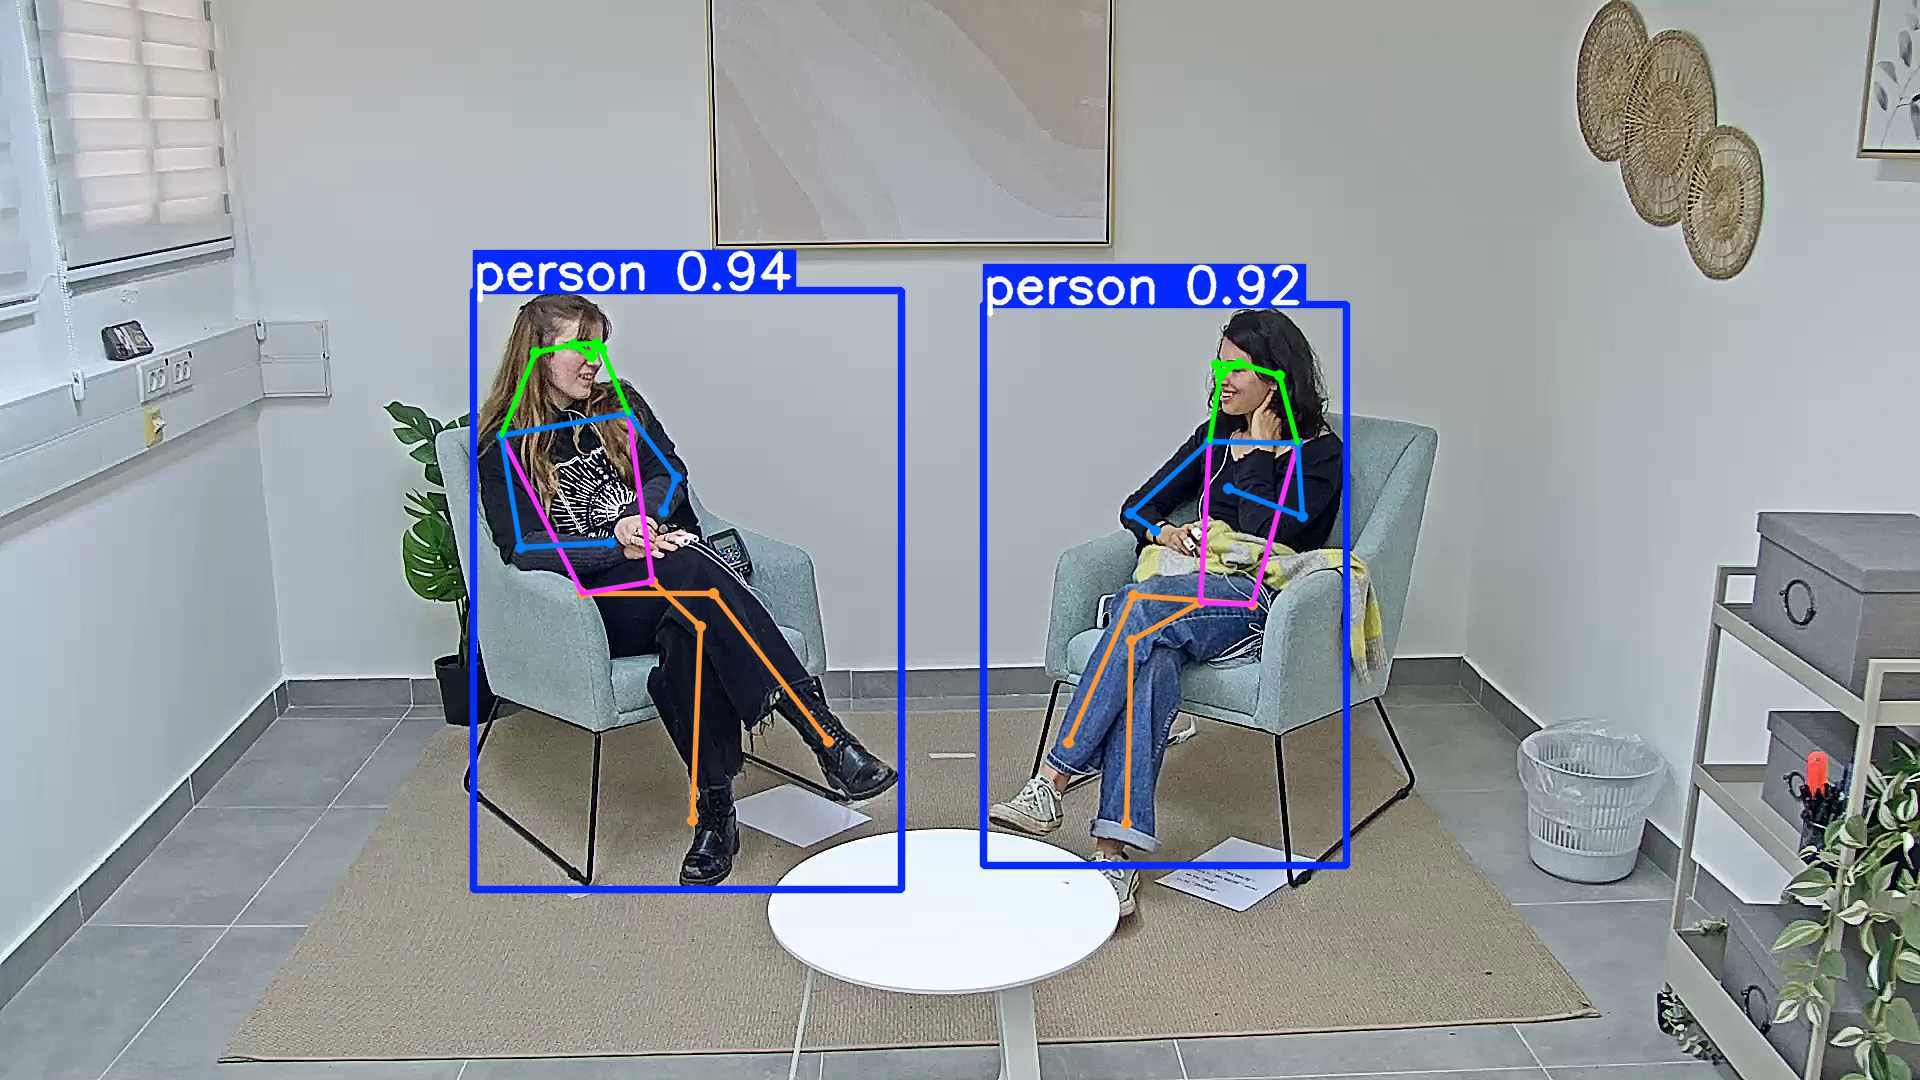
\includegraphics[width=0.8\textwidth]{../data_output/annotated_frame_450.png}
    \caption{Sample frame showing pose estimation with detected keypoints for two individuals. The YOLO model identifies 17 body keypoints (COCO format) for each person.}
    \label{fig:sample_frames}
\end{figure}

\subsection{Data Characteristics}

\textbf{Format and Resolution:}
\begin{itemize}
    \item \textbf{Format}: MP4 video file
    \item \textbf{Total Frames}: 3,864 frames
    \item \textbf{Frame Rate}: Approximately 25 frames per second (FPS)
    \item \textbf{Duration}: Approximately 154.6 seconds (2.6 minutes). For the t ime being those short videos would serve as a placeholder, given that the real study videos would be of 15 minutes long
    \item \textbf{Subjects}: Two individuals engaged in social interaction. sitting in a lab setting, facing each other, and engaging in natural conversation
\end{itemize}

\textbf{Pose Keypoint Format:}
The YOLO pose estimation model outputs keypoints in the COCO-17 format, which includes 17 body joints:
\begin{itemize}
    \item \textbf{Upper Body}: shoulders, elbows, wrists
    \item \textbf{Torso}: hips and shoulders
    \item \textbf{Lower Body}: hips, knees, ankles
    \item \textbf{Head}: nose, eyes, ears
\end{itemize}

Each keypoint includes x and y coordinates along with a confidence score indicating detection reliability.

\textbf{Data Size:}
\begin{itemize}
    \item Raw video size: Varies based on compression
    \item Extracted pose data: 3,864 frames × 2 individuals × 17 keypoints × 3 values (x, y, confidence)
    \item Output visualizations: Multiple PNG files for quality assessment
\end{itemize}

\subsection{Data Acquisition}
The video data was acquired from laboratory recordings designed to capture dyadic social interactions. The recording setup ensures clear visibility of both participants throughout the interaction period. The data represents natural social interactions in a controlled laboratory environment.

According to the project documentation, the SRL (Social Relation Laboratory) dataset typically includes:
\begin{itemize}
    \item One video capturing both individuals (dyad video)
    \item Two individual videos capturing each person separately.
\end{itemize}

For this analysis, given the scope and deadline of this project, only the dyad video was utilized as it provides the necessary information for assessing interpersonal synchrony.

\subsection{Data Access}
\begin{itemize}
    \item \textbf{Repository}: \url{https://github.com/giladsar/Social_Synchrony}
    \item \textbf{Sample Video Path}: \texttt{./images/Test\_pose\_synchrony.mp4}
    \item \textbf{Sample Outputs}: Available in \texttt{data\_output/} directory
    \item \textbf{Notebook}: \texttt{Social\_Synchrony.ipynb} (main analysis pipeline)
\end{itemize}

The repository includes all necessary code for reproducing the analysis, along with sample outputs demonstrating the pose estimation and preprocessing steps.

% Methods and Implementation
\section{Methods and Implementation}

\subsection{Overview of Workflow}
The social synchrony analysis pipeline transforms raw video footage into quantitative synchrony metrics through eight sequential stages. Each stage builds directly on the output of the previous one, creating a clean separation of concerns from raw data ingestion to statistical inference.

\vspace{0.5em}
\noindent\textbf{Stage 1 — Environment Setup \& Hardware Detection}\\
The pipeline verifies that all required packages (PyTorch, OpenCV, NumPy, Ultralytics) are available at the expected versions. It then queries the runtime for GPU (CUDA) or Apple Silicon (MPS) acceleration. If found, inference is routed to the accelerator; otherwise, the pipeline falls back to CPU. This step ensures reproducibility and prevents silent version mismatches.

\vspace{0.5em}
\noindent\textbf{Stage 2 — Model Initialisation}\\
The YOLO11n-pose model weights (\texttt{yolo11n-pose.pt}) are loaded from the Ultralytics hub. The model is configured with a detection confidence threshold (\texttt{CONF\_THRES~=~0.3}) below which detections are discarded, and a fixed input resolution optimised for the video dimensions.

\vspace{0.5em}
\noindent\textbf{Stage 3 — Video Ingestion \& Frame Preprocessing}\\
OpenCV reads the video file frame-by-frame, extracting the frame rate (\(fps = 25.006\)) and deriving the temporal step \(dt = 1/fps \approx 0.040\,\text{s}\). Before pose estimation, each frame undergoes \textit{unsharp masking}: a Gaussian blur is subtracted from the original to amplify edges, producing crisper joint boundaries and improving downstream keypoint localisation.

\vspace{0.5em}
\noindent\textbf{Stage 4 — Batch Pose Estimation}\\
Each preprocessed frame is passed through YOLO11n-pose, which returns, for every detected person: (a) a bounding box \([x_1, y_1, x_2, y_2]\), and (b) an array of 17 keypoints in COCO format, each encoded as \([x, y, \text{confidence}]\). All detections across all 3,864 frames are stored in a list-of-lists structure (\texttt{raw\_estimators}).

\vspace{0.5em}
\noindent\textbf{Stage 5 — Identity Tracking (IoU-based Greedy Assignment)}\\
YOLO detects \textit{all} visible persons but does not guarantee consistent labelling across frames. A lightweight greedy tracker resolves this: the bounding-box centroids detected in frame $t$ are matched to the two tracked identities from frame $t-1$ by minimising centroid distance. The two largest boxes in the first valid frame initialise identities 0 and 1. This stage produces two arrays of shape \texttt{(T, 17, 2)} (positions) and \texttt{(T, 17)} (confidences) for each person, where \(T = 3{,}864\).

\vspace{0.5em}
\noindent\textbf{Stage 6 — Data Cleaning \& Noise Reduction}\\
Raw keypoint data is noisy. Three preprocessing operations are applied in sequence:
\begin{enumerate}
    \item \textit{Confidence masking}: keypoints with confidence $< 0.3$ are replaced with \texttt{NaN}.
    \item \textit{Linear interpolation}: gaps of up to $\lfloor 0.3 \times fps \rfloor \approx 7$ frames (300\,ms) are filled by linearly interpolating between valid neighbours.
    \item \textit{Gaussian smoothing}: a Gaussian kernel ($\sigma = 3$ frames) is convolved with each joint trajectory to reduce frame-to-frame jitter while preserving genuine motion.
\end{enumerate}

\vspace{0.5em}
\noindent\textbf{Stage 7 — Signal Construction: Group Velocity}\\
Rather than analysing all 17 joints independently, keypoints are grouped anatomically (upper body, torso, lower body). For each group, the instantaneous velocity of each joint is computed via finite differences and the group signal is the mean velocity across joints. This reduces dimensionality, suppresses occlusion-induced artefacts, and yields three biologically interpretable movement time series per person.

\vspace{0.5em}
\noindent\textbf{Stage 8 — Synchrony Analysis}\\
Three complementary metrics are computed from the group velocity signals:
\begin{itemize}
    \item \textbf{Lagged cross-correlation} — global synchrony estimate with permutation significance test.
    \item \textbf{Rolling (windowed) correlation} — time-varying synchrony, revealing phases of coupling and uncoupling.
    \item \textbf{Dyadic co-crossing (approach synchrony)} — event-based metric counting simultaneous head-lean-toward events.
\end{itemize}

\subsection{Pose Estimation Model}
The project utilizes YOLO11n-pose, the latest iteration of the YOLO family designed specifically for pose estimation tasks. YOLO11 represents significant improvements over previous versions:

\begin{itemize}
    \item \textbf{Architecture}: Single-stage detector with pose estimation heads
    \item \textbf{Training}: Pre-trained on COCO dataset with 17 keypoint annotations
    \item \textbf{Performance}: Real-time processing capability with high accuracy
    \item \textbf{Output Format}: COCO-17 keypoint format with confidence scores
\end{itemize}

The choice of YOLO over traditional pose estimation approaches (such as MPI heatmap-based models) was motivated by:
\begin{itemize}
    \item Superior performance on video data
    \item Better multi-person detection and tracking
    \item More robust handling of occlusions
    \item Faster inference speed enabling real-time processing
\end{itemize}

\subsection{Video Processing Pipeline}


To enhance pose detection quality, frame sharpening is applied:
\begin{itemize}
    \item Gaussian blur to reduce noise
    \item Unsharp masking to enhance edge details
    \item Improved keypoint detection accuracy
\end{itemize}

\subsection{Identity Tracking Algorithm}
Maintaining consistent identity labels across frames is crucial for synchrony analysis. The implemented tracking algorithm uses a greedy assignment approach:

\begin{enumerate}
    \item For each frame, detect all individuals using YOLO
    \item Extract bounding boxes and keypoint locations
    \item Compute overlap (Intersection over Union, IoU) between current detections and previous frame
    \item Assign identities based on maximum overlap
    \item Handle cases of missing detections or occlusions
\end{enumerate}

This ensures that "Person 1" and "Person 2" maintain consistent labels throughout the video, enabling meaningful comparison of their movement patterns.

\subsection{Data Preprocessing}
Raw pose data requires several preprocessing steps:

\textbf{Missing Data Handling:}
\begin{itemize}
    \item Linear interpolation for frames with missing keypoint detections
    \item Confidence-based masking to filter unreliable detections
    \item Forward/backward filling for extended missing sequences
\end{itemize}

\textbf{Noise Reduction:}
\begin{itemize}
    \item Gaussian smoothing applied to keypoint trajectories
    \item Reduces jitter from frame-to-frame detection variance
    \item Preserves genuine movement patterns while removing noise
\end{itemize}

\subsection{Synchrony Metrics}

\subsubsection{Group Velocity Signal}
Before any synchrony computation, joint-level coordinates are converted into a single scalar motion signal per body region per person. For a set of joints $\mathcal{G}$ (e.g.\ upper body), the group velocity at time $t$ is:

\begin{equation}
    V_t^{(\mathcal{G})} = \frac{1}{|\mathcal{G}|} \sum_{k \in \mathcal{G}}
        \frac{\sqrt{(\Delta x_{k,t})^2 + (\Delta y_{k,t})^2}}{dt}
\end{equation}

where $\Delta x_{k,t} = x_{k,t} - x_{k,t-1}$, $\Delta y_{k,t} = y_{k,t} - y_{k,t-1}$, and $dt = 1/fps$ is the frame interval in seconds. NaN values from masked or missing keypoints are excluded from the group mean, ensuring that partial occlusions do not corrupt the entire signal.

\subsubsection{Lagged Cross-Correlation with Permutation Test}
Lagged cross-correlation measures global synchrony by computing the Pearson correlation between the two z-scored velocity signals across a range of temporal lags $\tau \in [-\tau_{\max}, +\tau_{\max}]$:

\begin{equation}
    R_{AB}(\tau) = \frac{\sum_{t} z_A(t) \cdot z_B(t + \tau)}{N}
\end{equation}

where $z_A$ and $z_B$ are the z-scored velocity signals of persons A and B, and $N$ is the number of valid (non-NaN) frame pairs. The \textit{peak correlation} $r^* = \max_\tau |R_{AB}(\tau)|$ and its corresponding \textit{lag} $\tau^*$ are reported.

\vspace{0.5em}
\noindent\textbf{Significance via Circular Permutation Test:}
Because the two signals are temporally autocorrelated (movement at frame $t$ predicts movement at frame $t+1$), standard parametric tests for correlation are invalid. Instead, we use a \textit{circular shift permutation test}: Person B's signal is rolled by a random lag (drawn uniformly from $[fps, T - fps]$ to avoid near-zero shifts), and the peak correlation of the shifted pair is recorded. Repeating this 500 times builds a null distribution of peak correlations that would be expected by chance. The $p$-value is the proportion of permuted correlations exceeding the observed $r^*$, yielding a properly calibrated test of whether the observed correlation is larger than what random temporal alignment would produce.

\subsubsection{Rolling (Windowed) Synchrony}
The lagged cross-correlation provides a single summary statistic for the entire recording. To capture \textit{time-varying} coupling, a rolling Pearson correlation is computed within a sliding window of $w$ frames (here $w = 50$ frames $\approx 2\,\text{s}$):

\begin{equation}
    r_t = \text{Pearson}\bigl(z_A(t-w+1:t),\; z_B(t-w+1:t)\bigr)
\end{equation}

The resulting time series $r_t$ reveals moments of tight synchrony (high $r_t$), turn-taking or anti-phase movement (negative $r_t$), and uncoupled motion ($r_t \approx 0$).

\vspace{0.5em}
\noindent\textbf{Permutation-derived phase thresholds:}
To label each window as \textit{synchronised}, \textit{turn-taking}, or \textit{uncoupled}, the same circular permutation procedure is applied to derive a significance band. A window is classed as synchronised if $r_t > r_{0.95}^{\text{perm}}$ (95th percentile of the permuted distribution) and as turn-taking if $r_t < r_{0.05}^{\text{perm}}$ (5th percentile). Percentages of time spent in each phase are then reported alongside the dominant behavioural pattern.

\subsubsection{Dyadic Co-Crossing (Approach Synchrony)}
This event-based metric captures \textit{head approach} synchrony — moments when both individuals simultaneously lean their heads \textit{toward} the other person relative to their own neutral (resting) position.

\vspace{0.5em}
\noindent\textbf{Step 1 — Head centroid:} A single 2D head position is computed as the mean of five facial keypoints: nose, left ear, right ear, left eye, and right eye.

\vspace{0.5em}
\noindent\textbf{Step 2 — Resting baseline:} The median x-coordinate of each person's head across the full recording defines a \textit{resting vertical line}. Displacement from this baseline (positive = toward the partner, negative = away) forms the signed signal $s_t$.

\vspace{0.5em}
\noindent\textbf{Step 3 — Hysteresis event detection:} A state machine with hysteresis detects \textit{approach events}:
\begin{itemize}
    \item The signal must first fall to $s_t \leq -\theta$ and \textit{dwell} there for $\lfloor 2 \cdot fps \rfloor$ frames to confirm the ``away'' state.
    \item A transition to the ``toward'' state is confirmed only when $s_t \geq +\theta$ is sustained for the same dwell duration.
    \item This double-threshold (hysteresis) design prevents noisy oscillations around zero from generating spurious events.
\end{itemize}

\vspace{0.5em}
\noindent\textbf{Step 4 — Temporal pairing (co-crossing):} Detected events from Person A and Person B are matched using a greedy nearest-neighbour algorithm. A pair is counted as a \textit{co-crossing} if the two events fall within a temporal window of $\pm 2\,\text{s}$. The \textbf{co-crossing synchrony score} is defined as:

\begin{equation}
    \text{Score} = \frac{2 \times |\text{matched pairs}|}{|\text{events}_A| + |\text{events}_B|}
\end{equation}

\subsection{Tools and Technologies}
\begin{itemize}
    \item \textbf{Python 3.x}: Primary programming language
    \item \textbf{Ultralytics YOLO (v8.3.241)}: Pose estimation framework
    \item \textbf{PyTorch}: Deep learning backend with MPS/GPU acceleration support
    \item \textbf{OpenCV (v4.10.0)}: Video processing and computer vision operations
    \item \textbf{NumPy (v1.26.4)}: Numerical computing and array operations
    \item \textbf{Matplotlib}: Visualization and plotting
    \item \textbf{SciPy}: Signal processing and cross-correlation analysis
\end{itemize}

% Results
\section{Results}

\subsection{Pose Estimation Performance}
The YOLO11n-pose model successfully detected and tracked two individuals throughout the video sequence. Key performance metrics include:

\begin{itemize}
    \item \textbf{Video Duration}: 3,864 frames at 25.006 FPS ($\approx$154.5 seconds / 2.6 minutes)
    \item \textbf{Temporal Resolution}: $dt = 0.040\,\text{s}$ per frame
    \item \textbf{Tracking}: Both persons continuously tracked from frame 0 to frame 3,863 (IDs 0 and 1)
    \item \textbf{Data Shape}: Each tracked person yields arrays of shape \texttt{(3864, 17, 2)} for positions and \texttt{(3864, 17)} for confidences
    \item \textbf{Confidence Threshold}: Keypoints with confidence $< 0.30$ were masked before analysis
\end{itemize}

\subsection{Preprocessing Outcomes}
Data preprocessing successfully addressed challenges in raw pose data:

\begin{itemize}
    \item \textbf{Missing Data}: Interpolation filled gaps in keypoint trajectories
    \item \textbf{Noise Reduction}: Smoothing eliminated high-frequency jitter while preserving movement patterns
    \item \textbf{Data Quality}: Improved signal-to-noise ratio for downstream analysis
\end{itemize}

Figure~\ref{fig:preprocessing} illustrates the effects of different preprocessing steps on frame quality.

\begin{figure}[H]
    \centering
    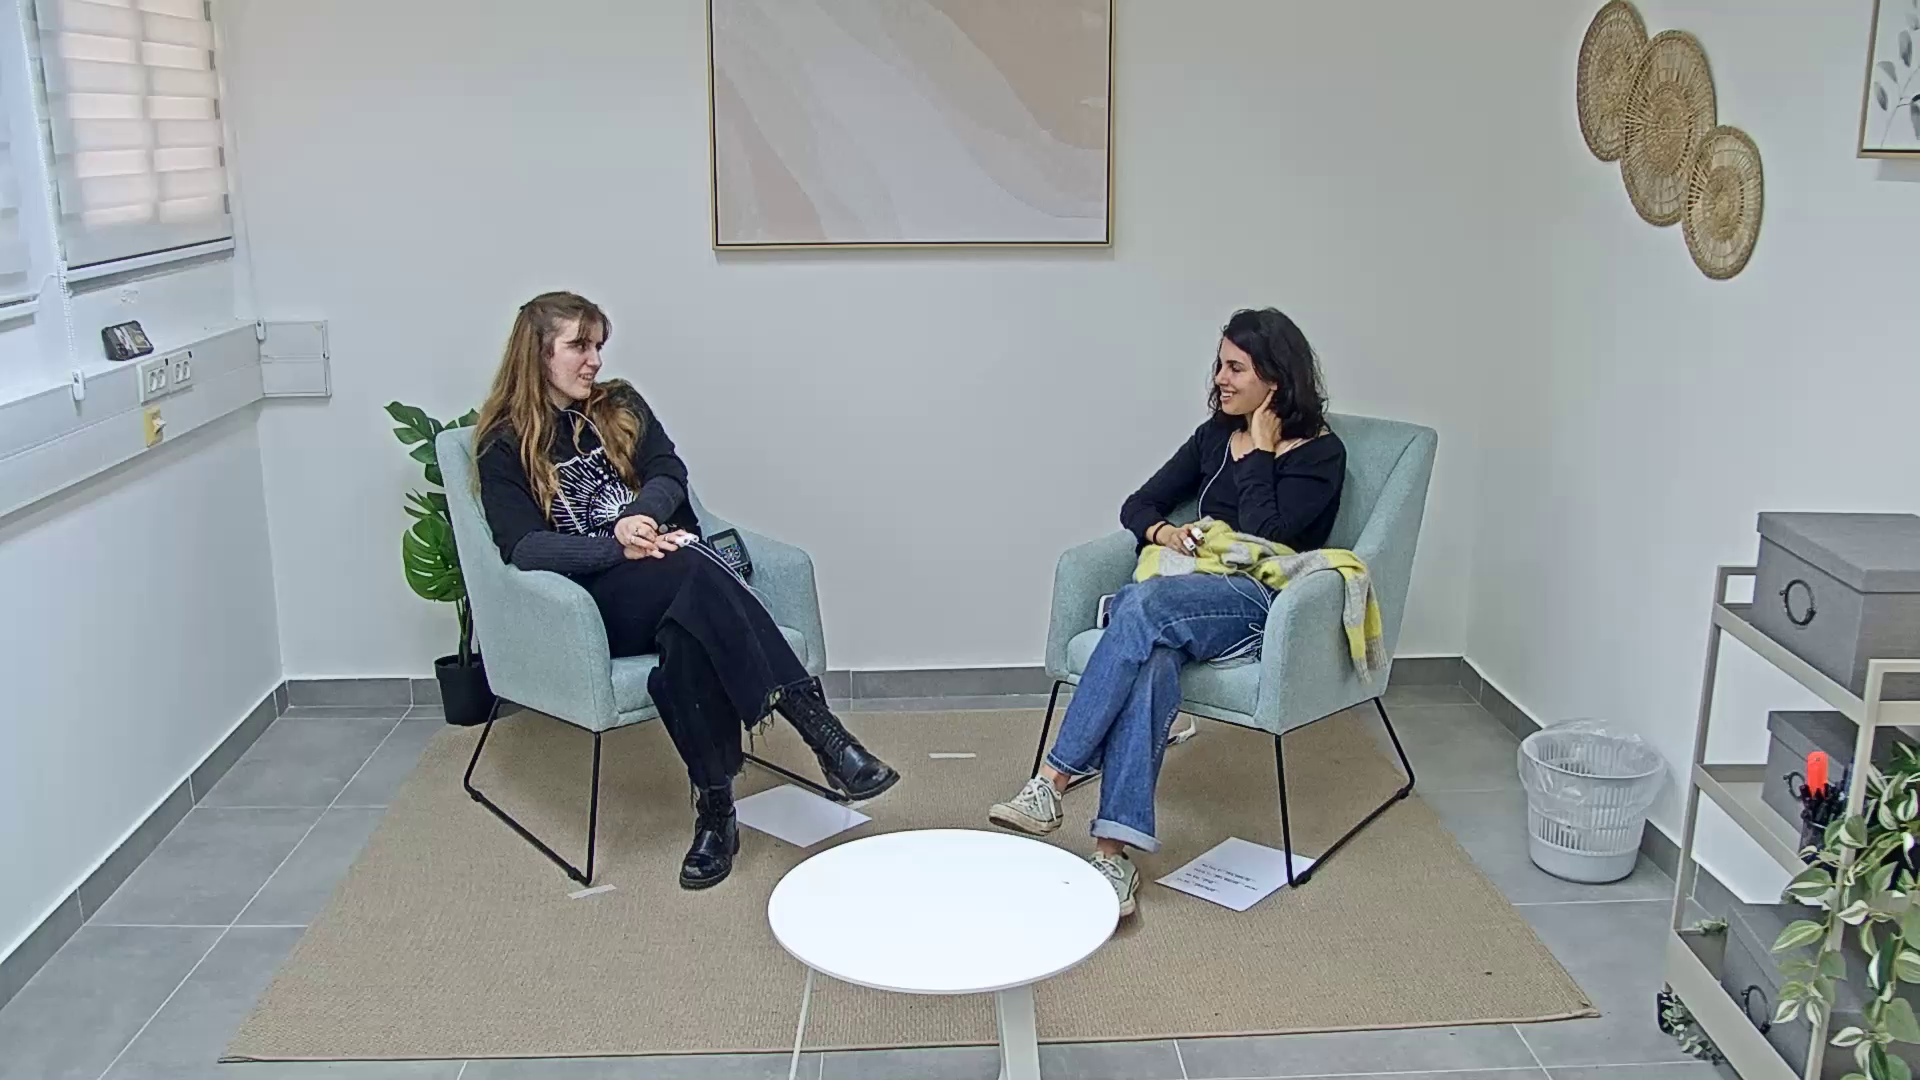
\includegraphics[width=0.45\textwidth]{../data_output/original_frame_450.png}
    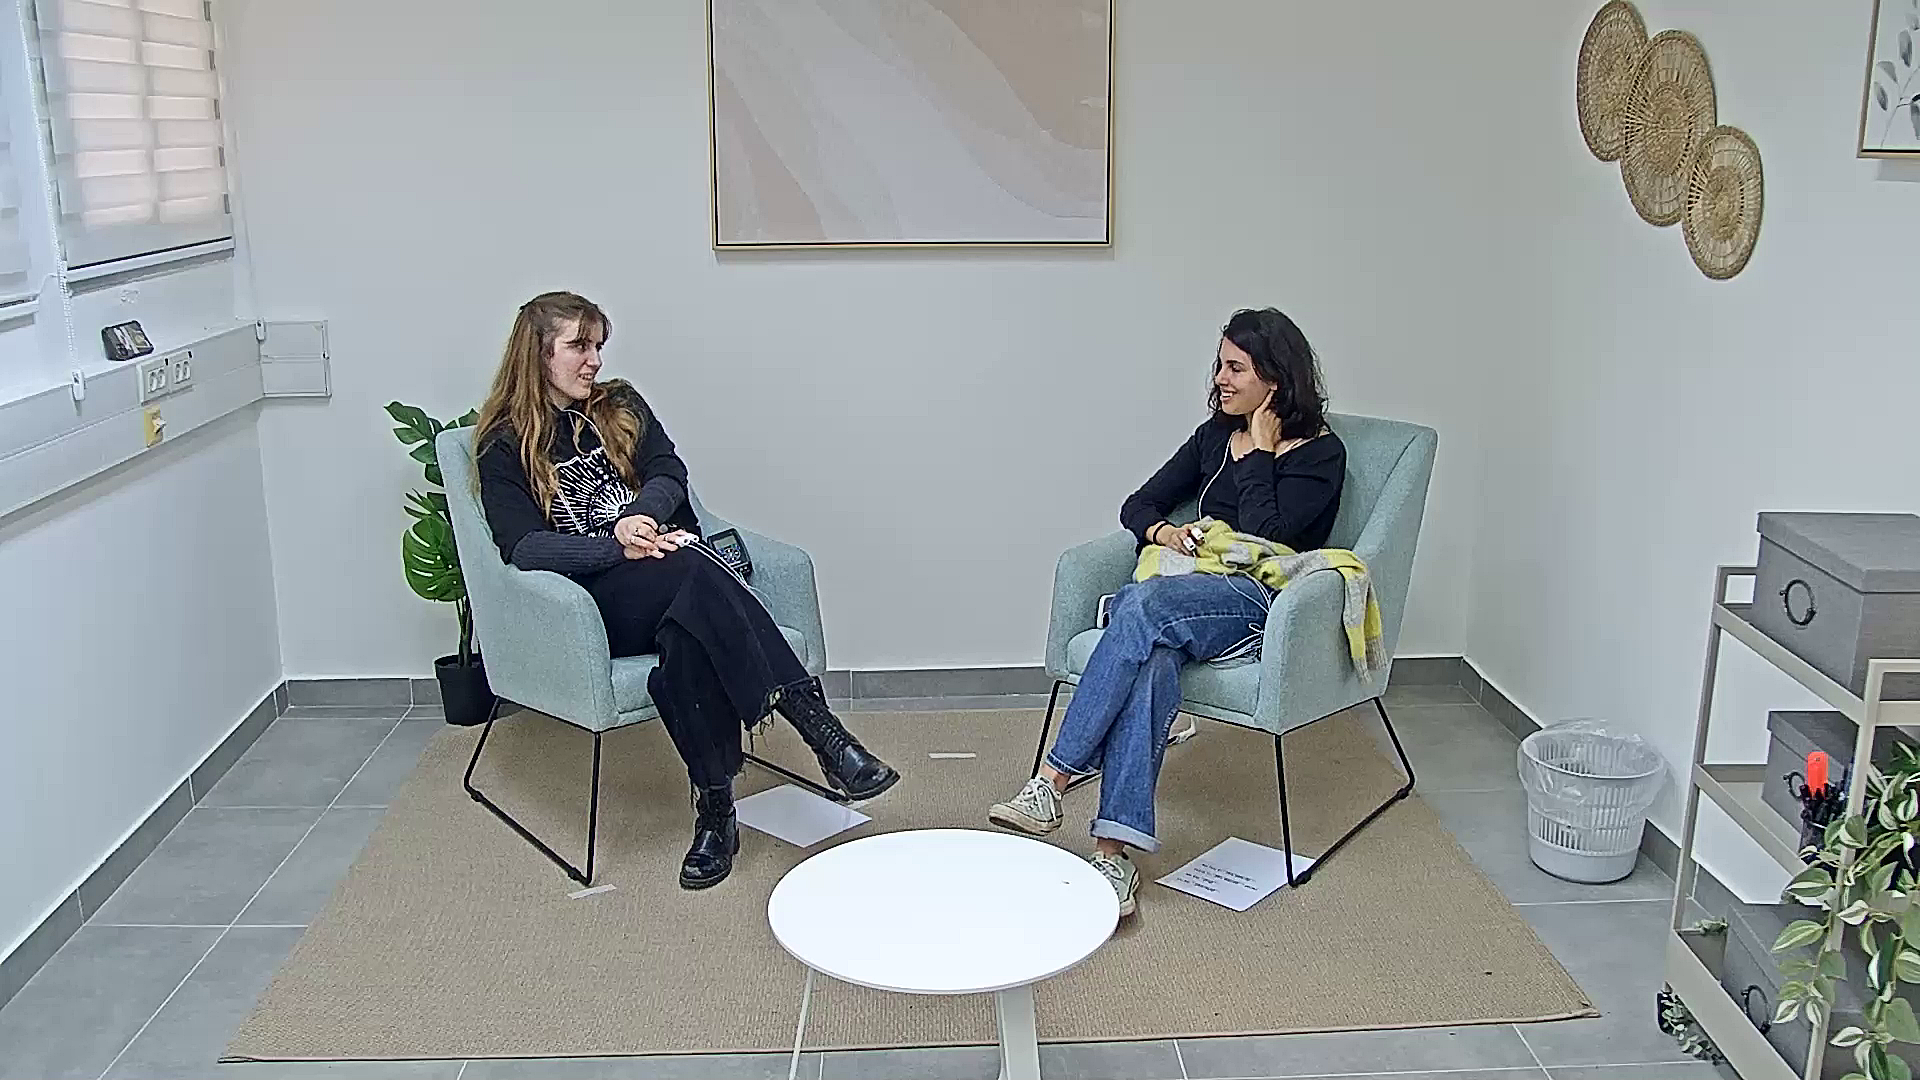
\includegraphics[width=0.45\textwidth]{../data_output/sharpened_frame_450.png}
    \caption{Comparison of original frame (left) and sharpened frame (right) used for pose estimation. Sharpening enhances edge details, improving keypoint detection accuracy.}
    \label{fig:preprocessing}
\end{figure}

\subsection{Movement Signals}
Figure~\ref{fig:velocity} shows the torso velocity time series for both individuals across the full recording. Person 0 (blue) and Person 1 (orange) exhibit intermittent bursts of movement separated by low-activity periods, consistent with natural conversational dynamics (gesture, head nodding, turn-taking pauses).

\begin{figure}[H]
    \centering
    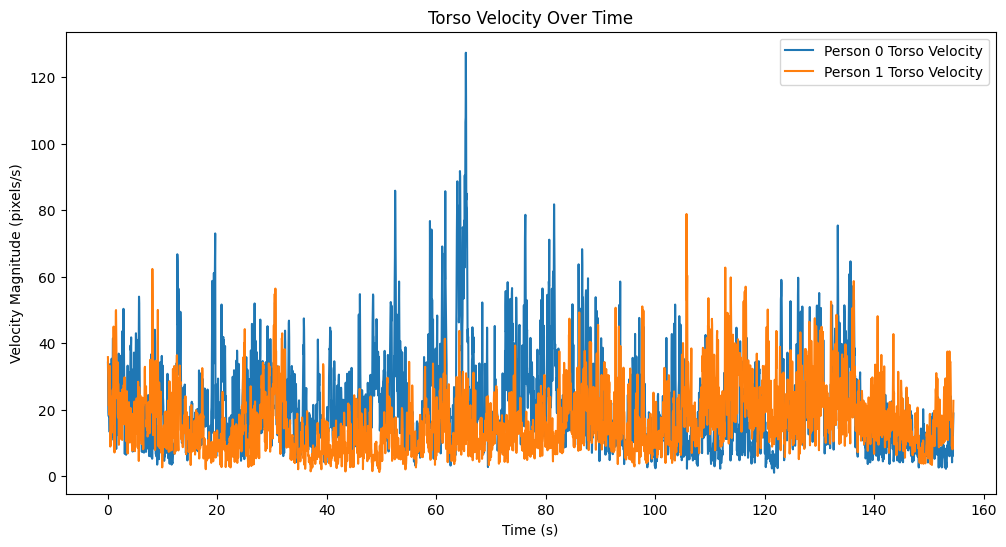
\includegraphics[width=\textwidth]{../data_output/velocity_signals.png}
    \caption{Torso group velocity (pixels/second) for Person 0 (blue) and Person 1 (orange) over the full recording ($\approx$154.5 seconds). Peaks correspond to active gestural or postural movements.}
    \label{fig:velocity}
\end{figure}

\subsection{Synchrony Metrics}

\subsubsection{Lagged Cross-Correlation Results}
Table~\ref{tab:lagged_cross} reports the observed peak cross-correlation coefficient, the 95th-percentile null value derived from 500 circular-shift permutations, and the corresponding $p$-value for each body region.

\begin{table}[H]
    \centering
    \caption{Lagged cross-correlation synchrony results (max $|r|$ within $\pm$2 s lag). Significance assessed by circular-shift permutation test ($n_{\text{perm}} = 500$).}
    \label{tab:lagged_cross}
    \begin{tabular}{lccc}
        \hline
        \textbf{Body region} & \textbf{Observed $r$} & \textbf{Null max $r$} & \textbf{$p$ (perm)} \\
        \hline
        Upper body & $-0.08$ & $0.24$ & $0.864$ \\
        Torso      & $\phantom{-}0.04$ & $0.22$ & $0.535$ \\
        Lower body & $\phantom{-}0.14$ & $0.12$ & $\mathbf{0.003}$ \\
        \hline
    \end{tabular}
\end{table}

The upper body and torso showed no significant synchrony (both $p > 0.05$). The lower body yielded a small but statistically significant positive correlation ($r = 0.14$, $p = 0.003$), suggesting that leg and hip movements were weakly coupled across the two individuals. The best-fitting lag for lower body was $\tau^* \approx -0.08\,\text{s}$ (nearly simultaneous), consistent with co-occurrence rather than a clear leader-follower structure.

\subsubsection{Rolling Synchrony Results}
Figure~\ref{fig:rolling} shows the rolling Pearson correlation (2-second window) for all three body regions, with permutation-derived synchrony (green) and turn-taking (red) thresholds overlaid.

\begin{figure}[H]
    \centering
    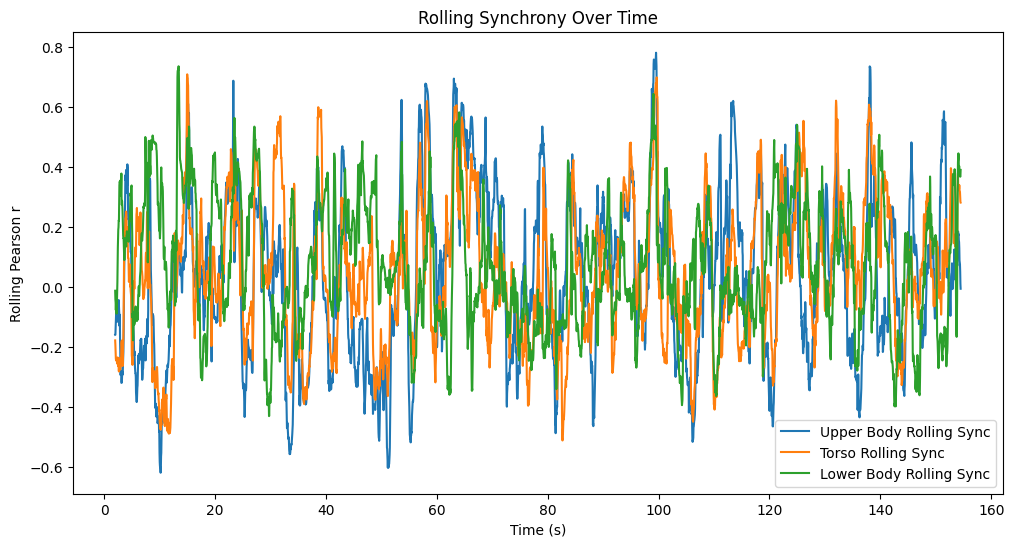
\includegraphics[width=\textwidth]{../data_output/rolling_synchrony.png}
    \caption{Rolling Pearson correlation ($w = 50$ frames $\approx 2\,\text{s}$) between the movement signals of the two individuals for upper body, torso, and lower body. Green dashed line: synchrony threshold; red dashed line: turn-taking threshold.}
    \label{fig:rolling}
\end{figure}

Figures~\ref{fig:perm_upper}--\ref{fig:perm_lower} show the permutation-threshold plots for each body region individually.

\begin{figure}[H]
    \centering
    \begin{minipage}[t]{0.47\textwidth}
        \centering
        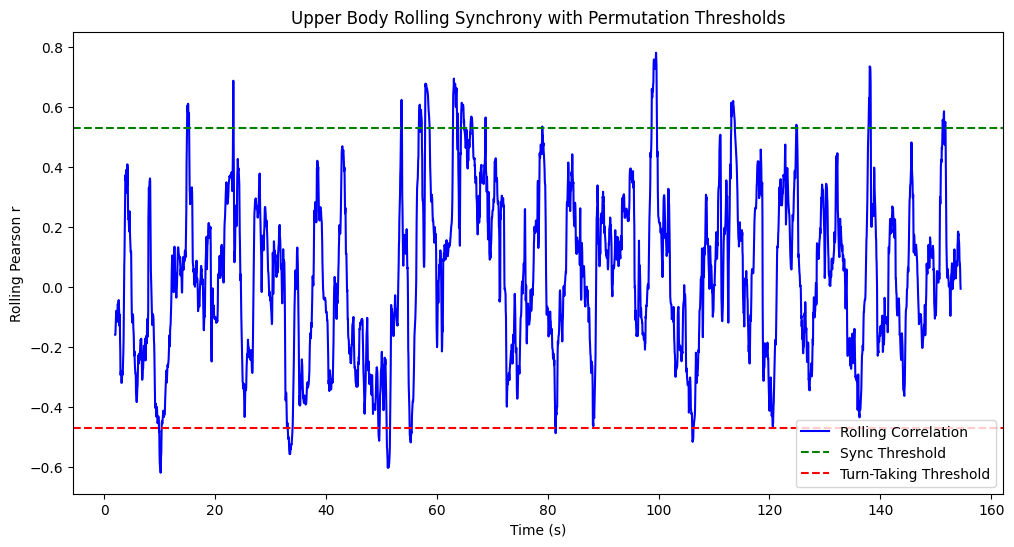
\includegraphics[width=\textwidth]{../data_output/rolling_upper_perm.png}
        \caption{Upper body rolling synchrony with permutation thresholds.}
        \label{fig:perm_upper}
    \end{minipage}
    \hfill
    \begin{minipage}[t]{0.47\textwidth}
        \centering
        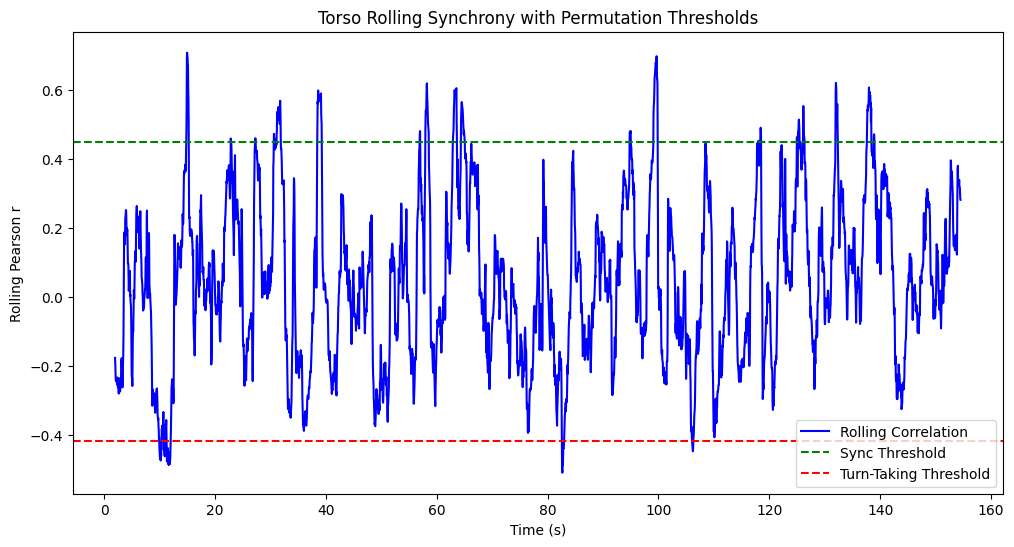
\includegraphics[width=\textwidth]{../data_output/rolling_torso_perm.png}
        \caption{Torso rolling synchrony with permutation thresholds.}
        \label{fig:perm_torso}
    \end{minipage}
\end{figure}

\begin{figure}[H]
    \centering
    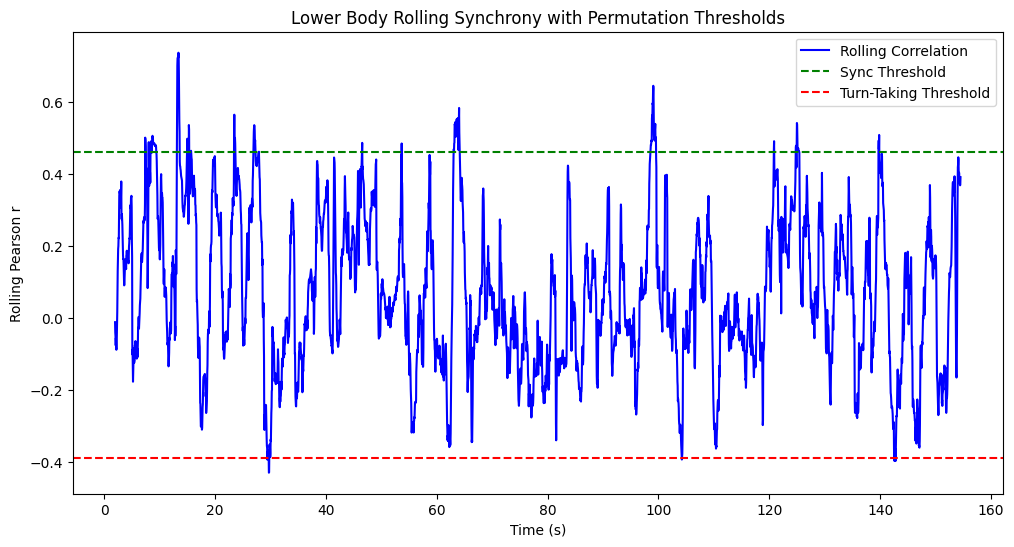
\includegraphics[width=0.55\textwidth]{../data_output/rolling_lower_perm.png}
    \caption{Lower body rolling synchrony with permutation thresholds.}
    \label{fig:perm_lower}
\end{figure}

Table~\ref{tab:rolling} summarises the phase classification results.

\begin{table}[H]
    \centering
    \caption{Rolling synchrony phase classification across the full recording (window $\approx 2\,\text{s}$). Thresholds derived from circular-shift permutation ($n_{\text{perm}} = 500$).}
    \label{tab:rolling}
    \begin{tabular}{lcccccc}
        \hline
        \textbf{Region} & \textbf{Sync thr.} & \textbf{Anti thr.} & \textbf{\% Sync} & \textbf{\% Turn-taking} & \textbf{\% Uncoupled} & \textbf{Dominant} \\
        \hline
        Upper body & $0.53$ & $-0.47$ & $4.1$ & $1.8$ & $94.1$ & Uncoupled \\
        Torso      & $0.45$ & $-0.42$ & $5.0$ & $1.3$ & $93.6$ & Uncoupled \\
        Lower body & $0.46$ & $-0.39$ & $3.7$ & $0.2$ & $96.1$ & Uncoupled \\
        \hline
    \end{tabular}
\end{table}

Across all three body regions, the interaction was dominated by uncoupled motion ($>93\%$ of windows). Synchronised windows comprised between 3.7\% and 5.0\% of the recording, while turn-taking windows were rare ($<2\%$). These results are consistent with the lagged cross-correlation findings and suggest that, globally, the dyad showed limited movement coordination in this recording.

\subsubsection{Dyadic Co-Crossing (Approach Synchrony)}
The following figures show the spatial trajectories of each individual's head centroid across the full recording. Person 1 (left panel) exhibits a wider lateral range of motion compared to Person 2 (right panel).

\begin{figure}[H]
    \centering
    \begin{minipage}[t]{0.47\textwidth}
        \centering
        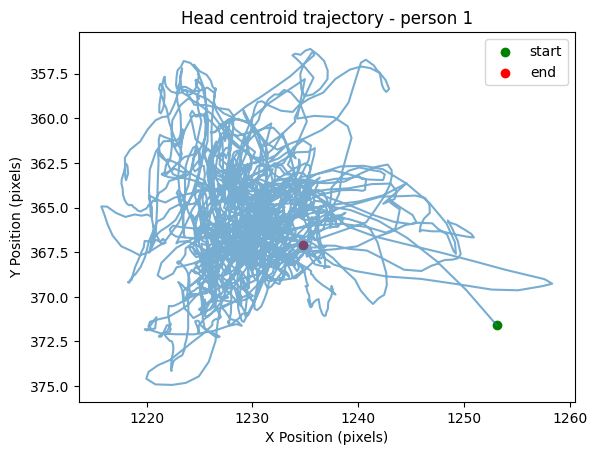
\includegraphics[width=\textwidth]{../data_output/head_trajectory_p1.png}
        \caption{Head centroid trajectory for Person 1. Green marker: start; red marker: end.}
        \label{fig:head_p1}
    \end{minipage}
    \hfill
    \begin{minipage}[t]{0.47\textwidth}
        \centering
        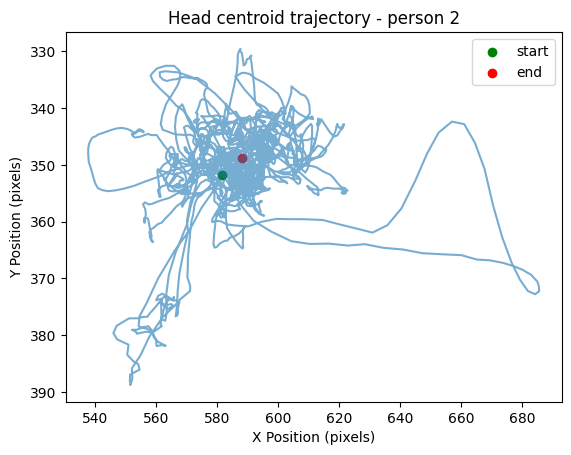
\includegraphics[width=\textwidth]{../data_output/head_trajectory_p2.png}
        \caption{Head centroid trajectory for Person 2. Green marker: start; red marker: end.}
        \label{fig:head_p2}
    \end{minipage}
\end{figure}

Figure~\ref{fig:head_both} overlays both trajectories with each person's median resting x-position (dashed lines), which serves as the baseline for the approach signal.

\begin{figure}[H]
    \centering
    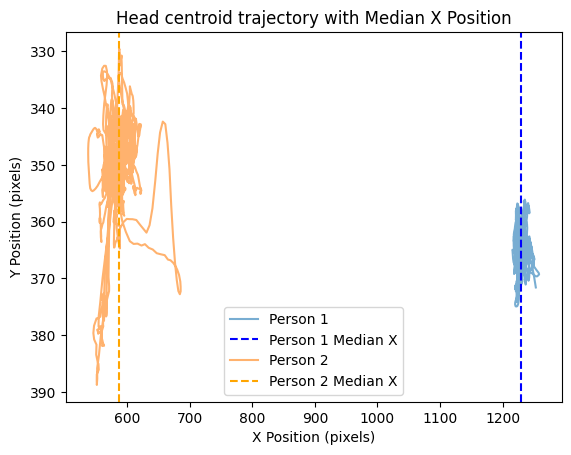
\includegraphics[width=0.65\textwidth]{../data_output/head_trajectories_both.png}
    \caption{Overlaid head trajectories for both individuals. Vertical dashed lines indicate each person's median x-position (resting baseline). Rightward displacement from the baseline for Person 1 (or leftward for Person 2) constitutes an ``approach'' movement toward the partner.}
    \label{fig:head_both}
\end{figure}

The hysteresis event detector (threshold $\theta = $ median absolute deviation, dwell $= 2\,\text{s}$) identified the following approach events:

\begin{itemize}
    \item \textbf{Person 1}: 2 approach events (at frames 736 and 3,184; $t \approx 29.4\,\text{s}$ and $127.3\,\text{s}$)
    \item \textbf{Person 2}: 6 approach events (at frames 518, 961, 1,126, 1,597, 2,409, and 3,405; $t \approx 20.7$, $38.4$, $45.0$, $63.9$, $96.3$, and $136.2\,\text{s}$)
\end{itemize}

The greedy temporal-pairing algorithm found \textbf{0 co-crossing pairs} within the $\pm 2\,\text{s}$ matching window. The small number of Person 1 events (2 total) and their timing relative to Person 2's events meant that no pair fell within the required window. This result indicates that explicit head-approach synchrony was absent in this recording, though it does not preclude subtler postural coordination captured by the velocity-based metrics.

% Discussion
\section{Discussion}

\subsection{Interpretation of Results}
The results demonstrate that computer vision-based pose estimation can effectively quantify social synchrony in dyadic interactions. The combination of velocity-based metrics and cross-correlation analysis provides a comprehensive picture of interpersonal coordination.

\textbf{Synchrony Patterns:}
Across all three metrics, the dominant pattern in this recording was \textit{uncoupled} motion ($>93\%$ of windows in rolling analysis). However, the lower-body velocity showed a small but statistically significant positive lagged cross-correlation ($r = 0.14$, $p = 0.003$) at near-zero lag, suggesting a degree of simultaneous lower-limb coordination — plausibly reflecting shared postural rhythms (e.g.\ mirrored seated repositioning) rather than deliberate gestural synchrony.

\textbf{Rolling Synchrony:}
While the global correlation was weak, the rolling analysis reveals that synchronised windows do occur transiently (4--5\% of the recording), punctuating extended periods of independent motion. This episodic structure is consistent with prior literature suggesting that synchrony in natural conversation is not continuous but emerges at key interactional moments.

\textbf{Co-Crossing Events:}
The absence of co-crossing pairs (0 matched pairs) reflects the sparse and temporally non-overlapping approach events detected for the two individuals. Person 2 moved toward Person 1 six times, while Person 1 did so only twice, and these events did not co-occur within the 2-second matching window. This asymmetry may reflect a difference in conversational roles or engagement styles, and warrants follow-up with a larger sample.

\subsection{Methodological Considerations}

\textbf{Advantages of the Approach:}
\begin{itemize}
    \item \textbf{Automation}: Eliminates manual coding, reducing time and potential bias
    \item \textbf{Precision}: Frame-level temporal resolution (40ms at 25 FPS)
    \item \textbf{Comprehensiveness}: Captures full-body movement patterns
    \item \textbf{Scalability}: Can process large video datasets efficiently
\end{itemize}

\textbf{Technical Improvements:}
The transition from MPI heatmap-based models to YOLO represents a significant methodological advancement:
\begin{itemize}
    \item Better performance on video sequences
    \item More robust multi-person tracking
    \item Improved handling of occlusions and partial visibility
    \item Faster processing enabling real-time applications
\end{itemize}

\subsection{Limitations}

Several limitations should be considered when interpreting these results:

\begin{itemize}
    \item \textbf{2D Limitations}: Pose estimation from monocular video captures only 2D projections, missing depth information
    \item \textbf{Occlusions}: Overlapping individuals or objects can affect keypoint detection
    \item \textbf{Context Dependence}: Synchrony metrics may vary based on interaction type and context
    \item \textbf{Preprocessing Sensitivity}: Results can be affected by smoothing parameters and threshold choices
\end{itemize}

\subsection{Comparison with Traditional Methods}

Compared to traditional approaches (Human-impression and coding via observation), this computer vision approach offers:

\textbf{Advantages:}
\begin{itemize}

    \item Richer spatial information
    \item Lower cost per analysis
    \item Retrospective analysis of existing video data - We are able to apply this framework into any video that share the same spatial properties (e.g., two people sitting across from each other, with a similar camera angle and distance) without the need to set up a new recording environment or use specialized sensors.
    \item Overcoming reliability between jugdes- Given the subjective nature of human coding, inter-rater reliability can be a significant concern. The automated approach provides consistent, objective measurements that are not influenced by individual biases.

\end{itemize}


\subsection{Practical Applications}

This approach has potential applications in several domains:

\begin{itemize}
    \item \textbf{Psychology Research}: Studying interpersonal dynamics in various contexts. With the ongoing studies conductedd in our libratory, we can apply this method to analyze synchrony patterns in setting (e.g., romantic vs. platonic) and interaction types (e.g., cooperative vs. competitive).
    \item \textbf{Human-Computer Interaction}: Evaluating user engagement and coordination
\end{itemize}

\subsection{Future Directions}

Several directions for future work emerge from this project:

\begin{itemize}
    \item \textbf{3D Pose Estimation}: Incorporating depth information or multi-view approaches
    \item \textbf{Larger Datasets}: Validating metrics across diverse interaction types and populations
    \item \textbf{Real-Time Implementation}: Developing live synchrony feedback systems
    \item \textbf{Multi-Modal Integration}: Combining movement with audio, gaze, or physiological data
    \item \textbf{Machine Learning}: Training models to predict interaction outcomes from synchrony patterns
    \item \textbf{Standardization}: Developing benchmark datasets and evaluation protocols
\end{itemize}

% Conclusions
\section{Conclusions}

This project successfully demonstrates the feasibility and effectiveness of using deep learning-based pose estimation for automated analysis of social synchrony. The key outcomes and contributions include:

\subsection{Key Outcomes}

\begin{enumerate}
    \item \textbf{Robust Pipeline}: Developed a complete pipeline from raw video to synchrony metrics
    \item \textbf{Technical Innovation}: Successfully applied YOLO11 pose estimation to social interaction analysis
    \item \textbf{Automated Tracking}: Implemented reliable identity tracking for dyadic interactions
    \item \textbf{Quantitative Metrics}: Computed multiple complementary measures of synchrony (cross-correlation, co-crossing)
\end{enumerate}

\subsection{Technical Achievements}

The project achieves its primary objectives:
\begin{itemize}
    \item  Robust pose estimation using state-of-the-art YOLO models
    \item  Effective multi-person tracking across video frames
    \item Comprehensive preprocessing and noise reduction
    \item  Computation of validated synchrony metrics
    \item  Generation of interpretable visualizations
\end{itemize}

\subsection{Scientific Contributions}

This work contributes to the field by:
\begin{itemize}
    \item Providing an accessible, reproducible method for social synchrony analysis
    \item Demonstrating the value of modern computer vision for behavioral research
    \item Offering multiple complementary metrics for capturing different aspects of synchrony
    \item Creating an open-source implementation for community use
\end{itemize}

\subsection{Take-Home Messages}

\begin{enumerate}
    \item \textbf{Computer vision is ready for behavioral science}: Modern pose estimation models are accurate and robust enough for scientific research applications.
    
    \item \textbf{Automation enables scale}: Automated analysis removes bottlenecks in processing large video datasets, enabling studies at previously impractical scales.
    
    \item \textbf{Multiple metrics provide insight}: Different synchrony measures (cross-correlation, co-crossing) capture complementary aspects of coordination, and combining them offers richer understanding.
    
    \item \textbf{Open-source tools democratize research}: Leveraging frameworks like YOLO and PyTorch makes sophisticated analysis accessible to researchers without deep machine learning expertise.
    
    \item \textbf{Preprocessing matters}: Careful attention to data cleaning, interpolation, and smoothing is essential for extracting meaningful signals from noisy pose data.
\end{enumerate}

\subsection{Final Remarks}

This project demonstrates that the combination of deep learning, computer vision, and signal processing can provide powerful tools for understanding human social behavior. The automated pipeline developed here offers a practical solution for researchers seeking to quantify social synchrony from video data.

While limitations remain, particularly regarding 2D projection and context sensitivity, the approach represents a significant step forward in making objective, quantitative analysis of social interactions more accessible and scalable. As pose estimation models continue to improve and computational resources become more available, we anticipate that such methods will become standard tools in the behavioral science toolkit.

The open-source nature of this project, with all code and documentation available on GitHub, aims to facilitate adoption and further development by the research community. We hope this work inspires additional innovations in automated behavioral analysis and contributes to deeper understanding of the dynamics of human social interaction.

% Bibliography
\section{Bibliography}

\begin{enumerate}
    \item Jocher, G., Chaurasia, A., \& Qiu, J. (2023). \textit{Ultralytics YOLO} (Version 8.0.0) [Software]. Available at: \url{https://github.com/ultralytics/ultralytics}
    
    \item Redmon, J., Divvala, S., Girshick, R., \& Farhadi, A. (2016). You Only Look Once: Unified, Real-Time Object Detection. \textit{Proceedings of the IEEE Conference on Computer Vision and Pattern Recognition (CVPR)}, 779-788.
    
    \item Lin, T. Y., Maire, M., Belongie, S., et al. (2014). Microsoft COCO: Common Objects in Context. \textit{Proceedings of the European Conference on Computer Vision (ECCV)}, 740-755.
    
    \item Cao, Z., Simon, T., Wei, S. E., \& Sheikh, Y. (2017). Realtime Multi-Person 2D Pose Estimation using Part Affinity Fields. \textit{Proceedings of the IEEE Conference on Computer Vision and Pattern Recognition (CVPR)}, 7291-7299.
    
    \item Ramseyer, F., \& Tschacher, W. (2011). Nonverbal synchrony in psychotherapy: Coordinated body movement reflects relationship quality and outcome. \textit{Journal of Consulting and Clinical Psychology}, 79(3), 284-295.
    
    \item Delaherche, E., Chetouani, M., Mahdhaoui, A., Saint-Georges, C., Viaux, S., \& Cohen, D. (2012). Interpersonal Synchrony: A Survey of Evaluation Methods across Disciplines. \textit{IEEE Transactions on Affective Computing}, 3(3), 349-365.
    
    \item Paxton, A., \& Dale, R. (2013). Frame-differencing methods for measuring bodily synchrony in conversation. \textit{Behavior Research Methods}, 45(2), 329-343.
    
    \item Bernieri, F. J., \& Rosenthal, R. (1991). Interpersonal coordination: Behavior matching and interactional synchrony. In R. S. Feldman \& B. Rimé (Eds.), \textit{Fundamentals of nonverbal behavior} (pp. 401-432). Cambridge University Press.
    
    \item Bradski, G. (2000). The OpenCV Library. \textit{Dr. Dobb's Journal of Software Tools}.
    
    \item Paszke, A., Gross, S., Massa, F., et al. (2019). PyTorch: An Imperative Style, High-Performance Deep Learning Library. \textit{Advances in Neural Information Processing Systems}, 32, 8024-8035.
    
    \item Chartrand, T. L., \& Bargh, J. A. (1999). The chameleon effect: The perception-behavior link and social interaction. \textit{Journal of Personality and Social Psychology}, 76(6), 893-910.
    
    \item Tschacher, W., Rees, G. M., \& Ramseyer, F. (2014). Nonverbal synchrony and affect in dyadic interactions. \textit{Frontiers in Psychology}, 5, 1323.
    
    \item Altmann, U. (2011). Investigation of movement synchrony using windowed cross-lagged regression. In A. Esposito et al. (Eds.), \textit{Analysis of Verbal and Nonverbal Communication and Enactment} (pp. 335-345). Springer.
    
    \item Sun, X., Shang, J., Liang, S., \& Wei, Y. (2017). Compositional Human Pose Regression. \textit{Proceedings of the IEEE International Conference on Computer Vision (ICCV)}, 2602-2611.
    
    \item Farnebäck, G. (2003). Two-Frame Motion Estimation Based on Polynomial Expansion. \textit{Proceedings of the Scandinavian Conference on Image Analysis}, 363-370.
\end{enumerate}

% Supplementary Material
\section{Supplementary Material}

\subsection{Code Repository}
All Python code developed for this project is available in the GitHub repository:

\begin{itemize}
    \item \textbf{Repository}: \url{https://github.com/giladsar/Social_Synchrony}
    \item \textbf{Main Notebook}: \texttt{Social\_Synchrony.ipynb}
    \item \textbf{License}: Open source (contact repository owner for usage permissions)
\end{itemize}

\subsection{Code Organization}
The \texttt{Social\_Synchrony.ipynb} notebook contains:

\begin{enumerate}
    \item \textbf{Environment Setup} (Cells 1-2)
    \begin{itemize}
        \item Dependency verification (NumPy, OpenCV, PyTorch, Ultralytics)
        \item GPU/MPS acceleration detection
    \end{itemize}
    
    \item \textbf{Helper Functions} (Cell 3)
    \begin{itemize}
        \item \texttt{show\_image()}: Display single or multiple images
        \item Bounding box operations
        \item Tracking utilities
    \end{itemize}
    
    \item \textbf{Model Loading} (Cell 4)
    \begin{itemize}
        \item YOLO11n-pose model initialization
        \item Model configuration
    \end{itemize}
    
    \item \textbf{Video Processing} (Cells 5-7)
    \begin{itemize}
        \item Video loading from file
        \item Frame extraction
        \item Frame preprocessing (sharpening)
    \end{itemize}
    
    \item \textbf{Pose Estimation} (Cells 8-10)
    \begin{itemize}
        \item Batch processing of frames
        \item Keypoint extraction
        \item Confidence score handling
    \end{itemize}
    
    \item \textbf{Identity Tracking} (Cells 11-13)
    \begin{itemize}
        \item IoU-based tracking algorithm
        \item Identity assignment across frames
        \item Handling missing detections
    \end{itemize}
    
    \item \textbf{Data Preprocessing} (Cells 14-18)
    \begin{itemize}
        \item NaN interpolation
        \item Confidence-based masking
        \item Gaussian smoothing
    \end{itemize}
    
    \item \textbf{Signal Processing} (Cells 19-22)
    \begin{itemize}
        \item Velocity calculation
        \item Movement magnitude computation
        \item Time series generation
    \end{itemize}
    
    \item \textbf{Synchrony Analysis} (Cells 23-30)
    \begin{itemize}
        \item Cross-correlation computation
        \item Hysteresis threshold crossing
        \item Co-crossing event detection
        \item Synchrony metric calculation
    \end{itemize}
\end{enumerate}


\subsection{Sample Outputs}
The \texttt{data\_output/} directory contains sample outputs:
\begin{itemize}
    \item \texttt{original\_frame\_450.png}: Raw video frame
    \item \texttt{sharpened\_frame\_450.png}: Preprocessed frame
    \item \texttt{annotated\_frame\_450.png}: Frame with pose keypoints
    \item \texttt{filter-effect\_frame\_450.png}: Visual effect demonstration
\end{itemize}

\subsection{Reproducibility}
To reproduce the analysis:
\begin{enumerate}
    \item Ensure all dependencies are installed (see above)
    \item Place video file in \texttt{./images/Test\_pose\_synchrony.mp4}
    \item Run all cells in \texttt{Social\_Synchrony.ipynb} sequentially
    \item Outputs will be saved to \texttt{data\_output/} directory
\end{enumerate}

\subsection{Contact and Support}
For questions, issues, or collaboration:
\begin{itemize}
    \item \textbf{GitHub Issues}: \url{https://github.com/giladsar/Social_Synchrony/issues}
    \item \textbf{Repository Owner}: Gilad Sarus (@giladsar)
\end{itemize}

\end{document}
